% Print optimised version of main.tex %

\documentclass[12pt, twoside]{report}
\usepackage[utf8]{inputenc}
\usepackage{titlesec}
\usepackage{geometry}
\usepackage{etoolbox}
\usepackage{xcolor}
\usepackage{enumitem}
\usepackage{amsmath}
\usepackage{amssymb}
\usepackage{xstring}
\usepackage{multicol}
\usepackage{tikz-dimline}
\usepackage{pdfpages}
\usepackage{setspace}

% To get current section name %
\usepackage{nameref}
\makeatletter
\newcommand*{\currentname}{\@currentlabelname}
\makeatother


% bibliography setup %
\usepackage[backend = biber,sorting = none]{biblatex}
\addbibresource{references.bib}


% On the spot flowchart creation %
\usetikzlibrary{shapes.geometric, arrows}
\tikzstyle{startstop} = [rectangle, rounded corners, minimum width=3cm, minimum height=1cm,text centered, draw=black, fill=red!30]
\tikzstyle{io} = [trapezium, trapezium left angle=70, trapezium right angle=110, minimum width=3cm, minimum height=1cm, text centered, draw=black, fill=blue!30]
\tikzstyle{process} = [rectangle, minimum width=3cm, minimum height=1cm, text centered, draw=black, fill=orange!30]
\tikzstyle{decision} = [diamond, minimum width=3cm, minimum height=1cm, text centered, draw=black, fill=green!30]
\tikzstyle{arrow} = [thick,->,>=stealth]


% Image setup %
\usepackage{graphicx}
\graphicspath{{./images/}}

% Link setup %
\usepackage{hyperref}
\hypersetup{colorlinks=true, linkcolor=black, urlcolor=black, citecolor = black,pdftitle={Analysis of stock market recommendations using computer vision}}


% caption layout for tables and images %
\usepackage{caption}
\usepackage{subcaption}
\captionsetup[table]{skip=7pt}
\captionsetup[figure]{skip=7pt}


\geometry{a4paper,left = 30mm,right = 20mm,top = 30mm,bottom = 22mm}
\textwidth = 160mm
\textheight = 245mm
\footskip = 7mm

% header formatting %
\usepackage{fancyhdr}
\pagestyle{fancy}
\fancyhf{}
\fancyhead[LE]{Chapter \thechapter}
\fancyhead[RE]{Section \thesection}
\fancyhead[CO]{\currentname}
\fancyfoot[CE,CO]{\thepage}


% Paragraph and line spacing %
\setlength{\parindent}{12mm}
\setlength{\parskip}{2.5mm}


% title formatting %
\titleformat{\chapter}[block]{\Huge\bfseries}{\chaptertitlename \ \thechapter}{0.5ex}
{
    \rule{\textwidth}{0pt}
    \vspace{1ex}
    \centering
}
\titlespacing{\thechapter}{0mm}{12mm}{12mm}


% Section formatting %
\titleformat{\section}[hang]{\fontsize{16}{16}\bfseries}{ \thesection}{1.4em}{}
\titlespacing{\thesection}{}{15mm}{15mm}

% Subsection formatting %
\titleformat{\subsection}[hang]{\fontsize{14}{14}\bfseries}{ \thesubsection}{1.4em}{}
\titlespacing{\thesubsection}{}{15mm}{15mm}

% First level ordered list %
\setlist[enumerate,1]{label=(\alph*)}


\begin{document}



\includepdf[pages=-]{auxiliary_pages}
\pagenumbering{roman}
\chapter*{Acknowledgements}

I am thankful to my institute Defence Institute of Advanced Technology (Pune) for considering my dissertation and providing help at all stages necessary during my work collecting information on my dissertation. \par

It gives me immense pleasure to express my deep and sincere gratitude to Dr.(Mr.) Dasari Srikanth (Dissertation guide) for his kind help and valuable advice during the development of the dissertation synopsis and his guidance and suggestions.
Apart from that, I would like to thank Mr Himanshu Chaudhary (co-guide), Manager from the Integrated Surveillance Department (ISD) of the Securities and Exchange Board of India (SEBI) for guiding me throughout this project and giving his valuable suggestions wherein necessary. I would like to express my deepest sense of gratitude to the employees of the Integrated Surveillance Department (ISD) and Information Technology Department (ITD) of SEBI who have put in their time and efforts to give additional guidance and suggestions during the project. \par
I would also like to thank the employees of Hewlett Packard Enterprise (HPE), a contractor of SEBI, who have allowed me to access their development environments, sophisticated hardware and cloud platforms, and associated tools and have been an immense help throughout this project. \par
I am deeply indebted to the Head of the Applied Mathematics Department, Dr. (Mr.) Somanchi VSSNVG Krishnamurthy, for giving me this valuable opportunity to do this project. I express my hearty thanks to him for his assistance, without which it would have been difficult to finish this project and review the project successfully.
I would like to convey my deep sense of gratitude to all the teaching and non-teaching staff for their constant encouragement, support, and selfless help throughout the dissertation work. It is my great pleasure to acknowledge the help and suggestions that I received from the Department of Applied Mathematics.

\setcounter{page}{6}
\chapter*{Abstract}



\renewcommand*\contentsname{Table of Contents}
\tableofcontents

\listoffigures

\listoftables

\chapter{Introduction}

\thispagestyle{empty} % no page number for introduction

\setcounter{page}{2} % remember counting now starts from 2
\pagenumbering{arabic} % style changes back to arabic

\section{Dissertation name and title}
My dissertation is titled \textbf{Analysis of stock market recommendations using computer vision}.

\section{Problem statement}

There is a large no. of daily broadcasts which take place throughout primetime (morning and evening) as well as outside of it. This project aims to digitize as well as summarise the recommendations cumulatively and present them to the end-user at the same time this project and its associated machine learning system are input to more sophisticated models for anomaly detection (in the context of violations in the securities market) at a later stage.

\section{Proposed solution}
The proposed solution is a deep learning model aimed at solving two fundamental machine learning problems at hand:
\begin{enumerate}

  \item	Object detection – Detect and classify important regions of interest in the frames of various NEWS broadcasts (or NEWS shows) i.e. regions having (but not restricted to) the name of the analyst/presenter, the recommendation being given, the company, commodity or the market segment being discussed and its corresponding listing symbol (if any), the various metrics of the recommendation such as stop loss, target price etc.

  \item  Optical Character Recognition (OCR) – Bilingual (English and Hindi) text obtained from the above regions of interest is passed onto sophisticated OCR models which have a text detection model and an actual language model(s) (corresponding to the concerned languages) working under the hood to obtain or extract the required information.

\end{enumerate}

The final output consists of a CSV (or) an excel file as required which summarises the above-obtained information.

\section{Scope and report contents}

Chapter \ref{chapter2} goes into a detailed discussion of the literature which has been studied while preparing this report. It includes several details such as (but not restricted to) how \textbf{YoLo} models or in general object detection models are evaluated and which performance metrics and common datasets are referred to for their speed and accuracy. It has additional details regarding how advanced deep learning models like \textbf{YoLov4} can be optimised for special use cases wherein necessary.
The complete work presented in this dissertation report is broadly divided into two parts which may be completed sequentially or parallelly and are described as follows. Additionally, the chapters to which they pertain to are also mentioned.

\begin{enumerate}
  \item Machine learning and computer vision: There are a total of 8 NEWS shows which are currently being targeted under this project. Machine learning used within this project is further divided into two parts: the one dealing with the recognition of various numerical parameters from the video frames of a broadcast (wherein active work is going on to increase efficiency as well as the accuracy of models) are random forest classifiers which have been trained on a large number of video frames which were earlier trained on \textbf{YoLov3} output (but needed additional training due to lesser accuracy) and templates followed by a much more robust and reliable framework i.e. YoLov4 which has been trained only for one NEWS show (i.e. \textit{PehlaSauda} from CNBC Awaaz). \par

  The second part of ML goes into OCR models wherein \textbf{no active work is being pursued} rather readymade models and OCR engines that are doing the job within tolerable error limits are being used. Both Tesseract – OCR and EasyOCR provided models have been used for this purpose and their performance metrics analysed. It should be noted that \textbf{no part of the report} goes into the details of the inner workings of the OCR models which are deep learning models in themselves. \par

  As opposed to standard ML projects wherein a considerable amount of time is used for training a particular model; this project uses more time and space to carry out a variety of image processing operations on the captured video frames. This includes histogram equalization, simple grey level transformations as well as complex erosion and dilation processes. After carrying out sufficient thresholding operations, these are fed into the ML models described above.

  The details for the above i.e. the process of collecting the data, preparing the data for training and testing and using appropriate deep learning models for the same are discussed in \ref{chapter3} in detail.

  \item Deployment into production: Rarely do data science projects in academia ever reach production and into a streamlined architecture. There are several reasons which prevent it from happening so. Such details, as well as reasons, have been given in brief in chapter \ref{chapter4}’s opening sections. \par
   Fortunately, for this project, the deployment of the data models falls within its current scope. All the ML models which would be trained and tested would be loaded onto the proprietary \textbf{Ezmeral MLOPs} platform by \textbf{HPE}. The servers for the same reside alongside the required hardware resources on SEBI’s internal servers. Doing this (without going into the details) would make the entire process streamlined i.e. the process of uploading videos, and training models on new data as soon as it is available and at the same time would decrease the manual work involved while doing so. As soon as the deployment has been completed, whether for all the NEWS shows or even a few of them, the internal server would be able to serve requests from within the organization domain (\textit{POST} methods with \textit{JSON} body) and at the same time would be able to abstract all the complex code and scripts running in the background. \par

   Apart from the MLOPs deployment, it is more desirable for SEBI to have a continuously running workflow that shall consist of processing a bulk or a batch of videos at once. A workflow about this has been deployed on a standalone virtual machine as a part of this project. Which projects require an MLOPs workflow and which don’t, as a result, have also been discussed in chapter \ref{chapter4}.
\end{enumerate}


Chapter \ref{chapter5} would then go on to discuss the various results which have been obtained at the end in terms of speed and accuracy of the YoLo models involved which metrics are suitable for evaluating projects spanning multiple ML models. Chapter \ref{chapter6} of the report would then finally present important conclusions drawn from the entire project.

\chapter{Literature review} \label{chapter2}

\section{YoLo – A brief discussion on v3 and v4 for real-time object detection}
YoLo standing for You Only Look Once is(are) a set of advanced deep learning models for real-time object detection. The focal point for YoLo is that it manages to perform bounding box regression and classification at the same time. The architecture or methodology which separates YoLo and other object detection frameworks is that other sophisticated frameworks (RCNN and even Fast RCNN) attempt to repurpose existing classifiers and localisers to perform object detection. They apply a single model to multiple locations within an image with variations in scale and other properties of the image multiple times. High scoring regions are labelled and classified accordingly. \par

YoLo frameworks take a drastically different approach: they divide the region into a large number of regions (or boxes) and simultaneously apply a single convolutional neural network to the entire image. The bounding boxes and associated probabilities are received at the output. These regions are then weighted according to these probabilities. The reason why this method supersedes other popular methods is that other neural network-based deep learning architectures (such as R-CNN) may end up using multiple network evaluations (in the order of thousands) on a single image that takes up a considerable amount of processing time. Additionally, YoLo models look at the entirety of the image during the detection phase because of which their predictions are based on the global context of the image. Although the differences don’t end here, these fundamental differences are enough to give YoLo a second to third order speed advantage over Fast R-CNN and R-CNN models. \par

The neural network for YoLo along with its entire compilation system is known as Darknet. A typical darknet run on an image, set of images, video or a real-time stream of image content (such as through a webcam) leads to the following three things as output:

\begin{itemize}
  \item The detected classes of objects (e.g. horse, car etc.)
  \item	The prediction confidence (e.g. $0.91$, $0.86$ etc.) and
  \item	The time it took to carry out the prediction or detection (e.g. $6$s, $12$s etc.)
  \item	Sophisticated high-level libraries will also produce the bounding boxes corresponding to each
\end{itemize}

\vspace{-0.2in}

Following is the output when a high-level library like \href{https://pypi.org/project/yolov4/}{yolov4} is used to process an image as shown below.

\begin{figure}[h]

\begin{center}
\begin{subfigure}{0.7\textwidth}
  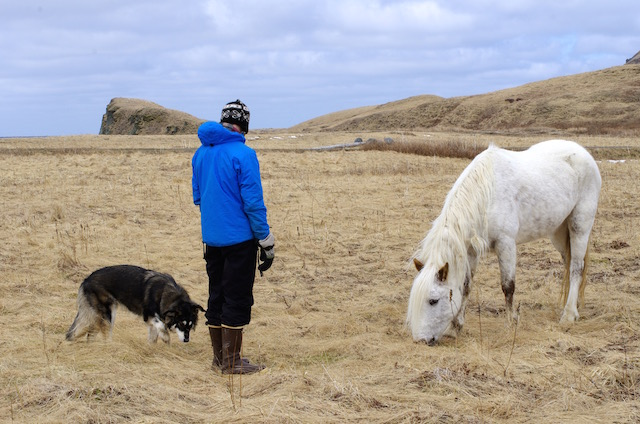
\includegraphics[width=\linewidth, height=5cm]{chapter2/person.jpeg}
  \caption{A sample image taken from the original Darknet \href{https://github.com/AlexeyAB/darknet}{github repository}}
  \label{fig:person_sub1}
 \end{subfigure} \\
 \begin{subfigure}{0.7\textwidth}
  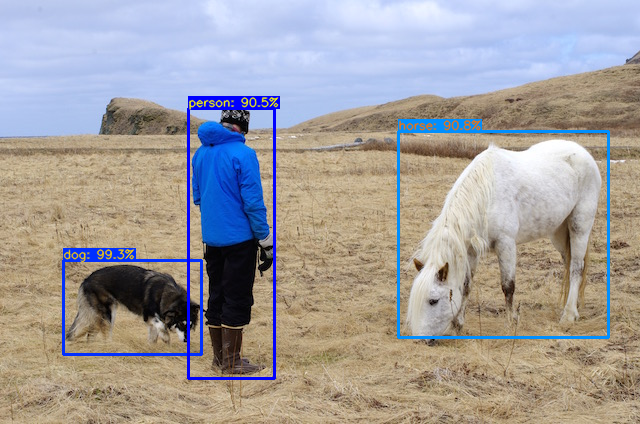
\includegraphics[width=\linewidth, height=5cm]{chapter2/personresult.png}
  \caption{Bounding boxes and detected objects in the image}
  \label{fig:person_sub2}
  \end{subfigure} \\
  \begin{subfigure}{0.7\textwidth}
   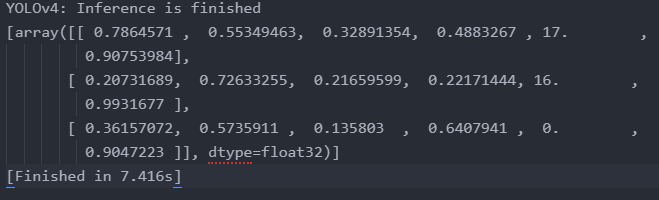
\includegraphics[width=\linewidth, height=5cm]{chapter2/personboxes.png}
   \caption{The bounding box coordinates obtained}
   \label{fig:person_sub3}
 \end{subfigure}

 \caption{A sample Darknet run on an image}
 \label{fig:person_ref}

\end{center}

\end{figure}



\subsection{YoLov3}
Joseph Redmond is credited with designing the original neural network architecture called Darknet. This was made using all low-level languages so that it could be made as flexible as it can be. This architecture went on to produce a series of computer vision wonders in the field of object detection named as YoLo: the original one, v2, v3 and then v4. Even YoLov5 has been developed (the first one to be developed by an organisation as opposed to an individual) at the time of writing this report. However, we won’t be discussing it here since it hasn’t been used in the concerned project. \par

YoLov3 is the first version using an objectivity score for the prediction of bounding boxes. It also proceeds to add further connections to the backbone of the entire architecture. Additionally, detections are also carried out at three levels of granularity which greatly increased the inferencing accuracy on smaller objects as well as objects/ smaller objects placed close to each other. There are some important parts or sections in YoLov3 which proves its robustness to a variety of real-life object detection scenarios. They relate to better bounding box prediction, class prediction, their feature extractor as well better prediction across multiple scales provided in the input. We would be discussing each of them in brief in the following paragraphs. \par

\subsubsection{Bounding box prediction}
Any bounding box in a prediction is represented by a set of four parameters namely $t_x$ and $t_y$: coordinates of the centre of the bounding box and its width and height represented by $t_w$ and $t_h$ respectively. In the event of the top left corner of the bounding box being displaced by $(c_x,c_y)$ respectively, the following overall changes are calculated in the dimensions (assume $p_w$ and $p_h$ are the width and height of the bounding box prior).
\begin{align*}
b_x &=  \sigma(t_x) + c_x \\
b_y &=  \sigma(t_y) + c_y \\
b_w &=  {p_w}e^{t_w} \\
b_h &=  {p_h}e^{t_h}
\end{align*}
Unlike previous systems (or previous YoLo versions), the training phase assigns an objectness score to each bounding box. This score equals one if the current bounding box overlaps a ground truth object to an extent greater than any other previously obtained bounding box. If any previously obtained bounding box doesn’t overlap the ground truth to a greater extent or overlaps only by a certain threshold (say $0.5$ as stated in this paper) then the objectness score is simply zero. Following is a representation of all the important dimensions which are involved in this process.

\begin{figure}
  \centering
  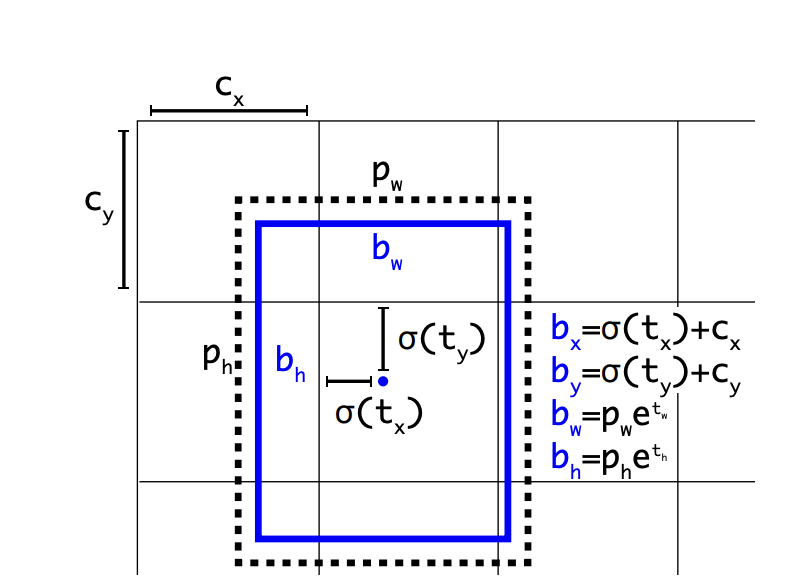
\includegraphics[scale=0.8]{chapter2/bounding_box.png}
  \caption{An illustration showing all the important bounding box dimesnions being used in YoLov3}
  \label{fig:bbox}
\end{figure}

\subsubsection{Class prediction}
SoftMax is one of the most common types of methods used for multi-label classification, however, the method has been leading to decrementing results for the class prediction accuracy in YoLov3 as well as has been unnecessary. Therefore, simple multiple logistic classifiers are being used for the purpose and binary cross-entropy has been used as a loss function. This different approach helped in the case of much larger and more sophisticated datasets such as the Open Images Dataset wherein labels may overlap frequently. SoftMax algorithm assumes that a single bounding box corresponds to exactly one label which is often not the case.

\subsubsection{Feature extraction}
Feature extraction in YoLov3 has been a hybridisation of the one in YoLov2, Darknet – 19 ($19$ convolutional layers) and another residual network. But the most important part of this network is shortcut connections which increase the size of the network significantly, however, continue to supersede ResNet variants in terms of efficiency. Since this leads to a total of $\boldsymbol{53}$ convolutional layers it's named Darknet-53.


\subsection{YoLov4 – improvements over YoLov3}

\section{Performance metrics for evaluating object detection models}

\section{Guidelines for a good YoLo project}
The following rules for a good project using YoLo are mere \textit{thumb – rules} and are not some strict guidelines to be followed and should be evaluated on a case to case basis for every project. Additionally, it should be noted that such rules may not be applicable for implementation in every object detection project. The following rules are bifurcated into those undertaken during the training and those in the testing (detection) phase.

\subsection{For training}

\begin{enumerate}
  \item The values of {\fontfamily{qcr}\selectfont random} should be set to $1$ in your  {\fontfamily{qcr}\selectfont .cfg} file which allows training for multiple image or video resolutions simultaneously.
  \item Every distinct object that is liable for detection must have an appropriate label in the dataset.
  \item Precision may be increased by keeping the height and width of images or video frames as a multiple of $32$.
  \item The training dataset should be such that every object to be detected corresponds to an exactly similar object in the training dataset. Similarity should be in terms of size, no. of classes to be detected ($c$), overall spatial orientation, overall illumination, augmentation (if any) etc. \par

  If the size of the training dataset is $N$ and the no. of classes is stated as above then training must run for at least $Nc$ iterations.
  \item Training datasets should have as many \textbf{positive} examples as there are \textbf{negative} examples (i.e. images which don’t have any object to be detected). Such negative examples shall return no bounding boxes when the detection or testing run is executed. These ensure an equal sensitivity of the model to both types of images as well as eliminate a lot of post-processing operations.
  \item Sometimes it is desirable to run your detections with the {\fontfamily{qcr}\selectfont -show\_imgs} option at the end so that it can be manually verified whether the predicted bounding boxes are correct or not. Seeing the detections and detecting some anomaly could be a direct implication of training runs going wrong or some inherent problem in the dataset.
\end{enumerate}


\subsection{For testing or detection}

\begin{enumerate}
  \item Increase network resolution in the same way as mentioned in 1. c.
  \item It should be noted that retraining is not required in the event of loss in your dataset or any other unintended corruption. Only the \textit{darknet} command should be available which can be used to perform detections using the pre-trained {\fontfamily{qcr}\selectfont .weights} file which was trained on the $416 \times 416$ resolution images.
  \item To further enhance the accuracy, dataset training must proceed onto higher multiples of  $32$ such as $608 \times 608$ or $832 \times 832$. In the event of a memory overflow ({\fontfamily{qcr}\selectfont Out of memory}), {\fontfamily{qcr}\selectfont subdivisions} in your {\fontfamily{qcr}\selectfont .cfg} file must be increased from $16$ to $32$ to $64$ and so on.
\end{enumerate}

\chapter{Methodology and development} \label{chapter3}

This chapter is the crux of the entire dissertation report and goes into all the nitty-gritty details of how the entire project with all its internal components is being developed.

\vspace{-0.1in}
\section{Video data} \label{vid_data}

The entirety of the video data was procured from a company called \href{clipbyte.com}{Clipbyte} which happens to be a premier Indian broadcasting and analysis corporation responsible for broadcast/telecast management as well as dedicated analysis of various broadcasts. It also tends to various other organisations which may need this data. \par

SEBI gave the contract to Clipbyte for providing videos of NEWS shows across a span of one and a half years and a total of $7$ NEWS shows. A summary of the entire data made available to SEBI at an undisclosed contract amount is enlisted below.

\begin{table}[h]
 \def\arraystretch{1.5}
 \centering
 \caption{Summary of videos available}
 \begin{tabular}{|c|c|}
  \hline
  NEWS show & Approximate no.\\
  \hline
  Buy Now Sell Now & $435$                   \\
  \hline
  Pehla Sauda & $435$                   \\
  \hline
  NSE Closing Bell & $435$                   \\
  \hline
  Bazaar Morning Call & $435$                   \\
  \hline
  Midcap Bazaar & $435$                 \\
  \hline
  Stock 20-20 & $326$                \\
  \hline
  Weekly Roundup & $37$              \\
  \hline
 \end{tabular}
 \label{tab:news_shows_acquired}
\end{table}

The amount of video data (primarily intended for bulk processing) amounts to roughly $1.08$ Tb in size and roughly $2137$ videos ranging from as small as $250$ Mb to videos of special broadcasts amounting to excess of $900$ Mb. The data was first loaded onto an intermediate server and then finally onto the state of the art SEBI Datalake server which is essentially a cloud platform. Later, the videos are fetched as required from the Datalake server itself for further processing. The current analysis is being done from scratch on the NEWS show Midcap Bazaar from the channel ZEE NEWS using sophisticated YoLov4 models and appropriate OCR engines. The data available only from this show is shown at a glance in the following table. The data available from other NEWS shows have a similar scale although they have not been shown here for convenience.

\begin{table}[h]
 \def\arraystretch{1.5}
 \centering
 \caption{Summary of video frames from Midcap Bazaar}
 \begin{tabular}{|c|c|}
  \hline
  Parameter & Number\\
  \hline
  Total videos & $266$                   \\
  \hline
  Total frames & $8584623$                   \\
  \hline
  Average frames per video & $32273$                   \\
  \hline
  Total frames in consideration @ FPS rate & $343371$                   \\
  \hline
  Average frames in consideration per video & $1291$                   \\
  \hline
  Total size of dataset & $5000$                   \\
  \hline
 \end{tabular}
 \label{tab:vid_data_tab}
\end{table}

\section{Data annotation and preparation}

As would be obvious from the above table, the reason for mentioning FPS rates and the average total number of frames available after filtering at the FPS rate is because only these frames would be available for the creation of a dataset as mentioned in the next section. Hence filtering is done @ $25$ FPS to obtain only $25$\textsuperscript{th} of the frames available originally. How much of these would be leading to the actual training and testing data is described in the following sections. \par

\subsection{Annotation}
This single-handedly is the biggest challenge in the entire project. Irrespective of the version of the YoLo framework being used, a large part of the efforts are concentrated on the creation of massive annotated datasets. The typical annotation involves marking out appropriate bounding boxes on regions of interest i.e. ROIs (as would be described in the subsequent sections) and labelling them appropriately in video frames. A typical broadcast which could be as small as $10$ mins. will lead to as many as $3000$ video frames which only after filtering as mentioned in the previous section need to be marked appropriately. This is a laborious task that has been simplified to some extent by the availability of readymade software like \href{https://roboflow.com/annotate}{Roboflow} \cite{rb2022}. \par

However, as told previously in the section \ref{mod_guides}, our dataset should be varied enough to develop or train a model which is robust to a variety of situations that could be encountered while parsing (a) frame(s) of a video from any NEWS show. Typical edge cases which must be looked at are enumerated below.
\begin{enumerate}
 \item In NEWS show broadcasts, it is common to have minor transitions between subsequent frames, this leads to intermediate blurring and de-blurring of important regions of interest. Our model should be in a position to identify them.
 \item The recommendations being given are available in a variety of formats with a variety of spatial arrangements. All should be annotated but should be labelled with the \textbf{same class}.
 \item Sometimes ROIs appear in the same way excepting their overall scale, they should be detected exactly in the same way as if it was their original size or scale.
\end{enumerate}
Following is an illustration of the annotation section of the Roboflow software.

\begin{figure}[h]
  \centering
  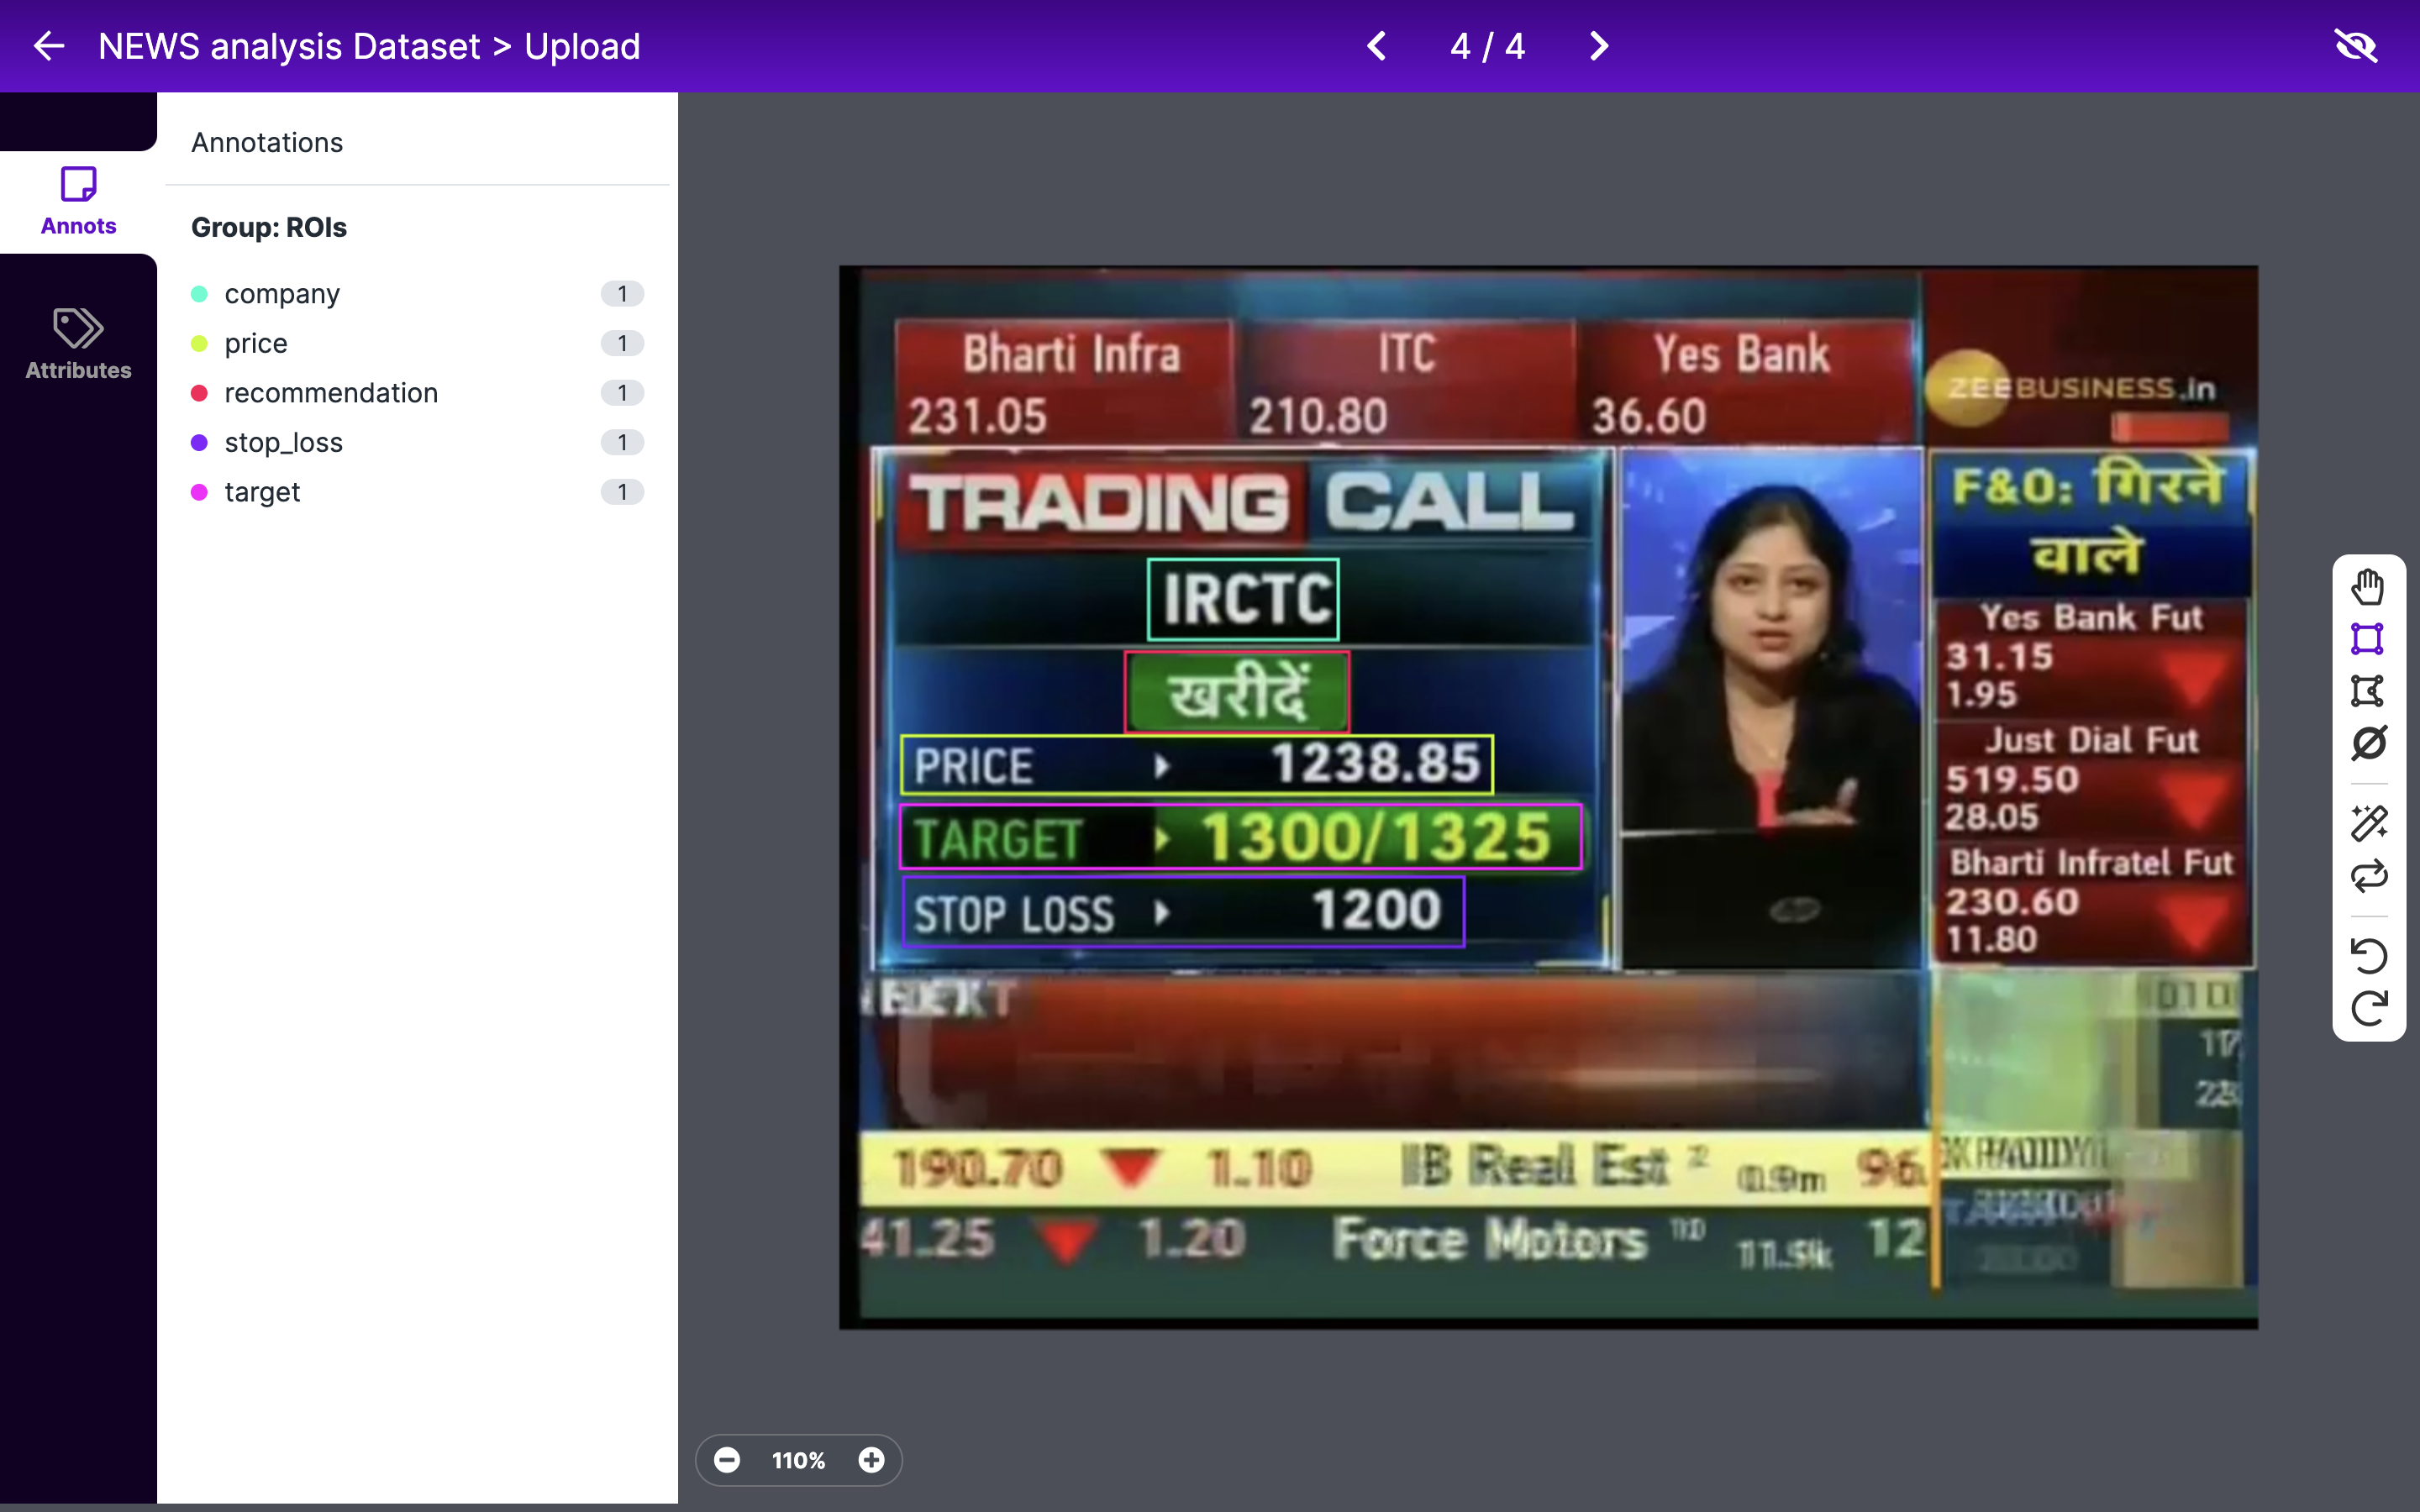
\includegraphics[scale=0.35]{chapter3/annotated_frame.png}
  \caption{The annotation screen in Roboflow clearly showing the bounding boxes made on a video frame and the appropriate classes listed on the left}
  \label{fig:annot_frame}
\end{figure}

\subsection{Data preparation for training and testing} \label{train_test}
Now we are going to boil down to the exact numbers involved in the training and testing dataset which would be summarised below. But before that, it should be noted from the table \ref{tab:vid_data_tab}, that the total images in the dataset are selected as $5000$. We can now write down a generic formula for the proportion of frames being taken from a video for annotation. Let $f_i$ be the number of frames obtained from the $i$\textsuperscript{th} video after filtering at the FPS rate and let $N$ be the total number of frames obtained across all videos in the dataset after filtering @ FPS rate i.e. $N = \sum f_{i}$. Then the proportion of its frames in the final dataset would be $\boldsymbol{F_{i} = \frac{f_{i}}{N}}$. \par

Apart from that, to adhere to the guidelines given in section \ref{mod_guides} and the edge cases described in the previous section, we need to generate a version of the dataset with each image going through a couple of additional processing steps. Such types of operations substantially increase model performance as well as drastically decrease inferencing times \cite{Joseph2021} \cite{Dwyer2020}. The operations are further divided into two parts namely \textbf{pre-processing} and \textbf{augmentation}.  The image pre-processing operations used are \textit{Resize} and \textit{Filter null}. The augmentation operations which were used are all bounding box augmentations such as \textit{crop}, \textit{blur}, \textit{brightness}, \textit{exposure} and \textit{noise}. Following is the final summary of our dataset for training and testing for a single NEWS show about its analysis as detailed in section \ref{yv4}.

\begin{table}[h]
 \def\arraystretch{1.5}
 \centering
 \caption{Summary of training dataset from Midcap Bazaar. Note: the no. of negative frames being much lesser than positive frames}
 \begin{tabular}{|c|c|}
  \hline
  Parameter & Value and unit \\
  \hline
  Frame size & $768 \times 576$                    \\
  \hline
  Training & $3500$ videos                   \\
  \hline
  Validation & $1000$ videos                 \\
  \hline
  Testing & $500$ videos                   \\
  \hline
  Positive frames (upto $7$ months) & $2566$                   \\
  \hline
  Negative frames (upto $7$ months) & $382$                   \\
  \hline
 \end{tabular}
 \label{tab:vid_train}
\end{table}

This software along with giving the capabilities to annotate a variety of subjects (pictures, videos, text etc.) produces the required weights file for the Yolo framework of any version (one through five). This when combined with the appropriate {\fontfamily{qcr}\selectfont \textbf{config}} file (a file containing the complete neural network-based configuration for the YoLo framework) is almost ready for compilation i.e. training and testing. One more additional file i.e. either a {\fontfamily{qcr}\selectfont \textbf{.data}} and/or {\fontfamily{qcr}\selectfont \textbf{names.list}} file would be required which would specify the names of the classes into which classification is supposed to occur. \par

In our case, the typical class names are used in a way that they represent what content they have in a particular frame e.g. \textbf{price}, \textbf{telecast date}, \textbf{stop loss}, textbf{recommendation} etc. The performance of the overall Python script in terms of the models used and still being worked upon are discussed in the subsequent chapters.

\section{ML/DL models}

This is the \textbf{\textit{heart and soul}} of the entire project. The methodologies mentioned here are only responsible for solving the two fundamental ML problems mentioned in chapter \ref{chapter1}. The NEWS shows are bifurcated into two parts consisting of $4$ and $3$ NEWS shows respectively. The first $4$ NEWS shows are viable for analysis in section \ref{yv3} and the latter set of shows are viable for analysis as detailed in section \ref{yv4}

\subsection{YoLov3 and random forest classifiers} \label{yv3}

It should be noted that the mere usage of the YoLov3 framework didn’t give a substantial number of accurate results so the training dataset was enhanced using \textbf{random forest classifiers} to obtain a substantial increase in percentage accuracy. The logic behind this is better illustrated through the following two flowcharts.

\begin{figure}[h]
 \centering
 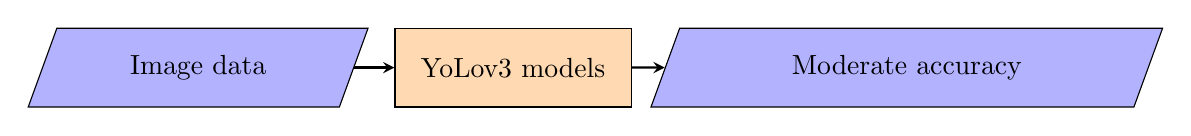
\begin{tikzpicture}[node distance=2cm]
  \node (input) [io] {Image data};
  \node (yolov3) [process, right of=input, xshift=2cm] {YoLov3 models};
  \node (output) [io, right of=yolov3, xshift=3cm] {Moderate accuracy};
  \draw [arrow] (input) -- (yolov3);
  \draw [arrow] (yolov3) -- (output);
 \end{tikzpicture} \\
 \vspace{1.5cm}
 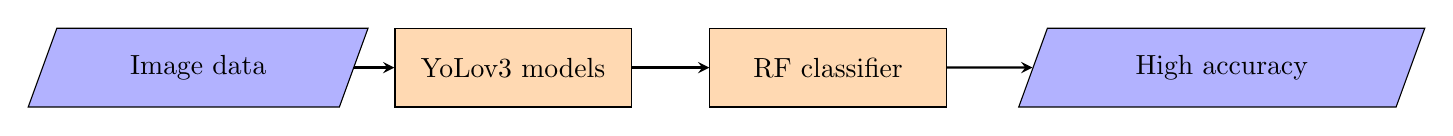
\begin{tikzpicture}[node distance=2cm]
  \node (input) [io] {Image data};
  \node (yolov3) [process, right of=input, xshift=2cm] {YoLov3 models};
  \node (rf) [process, right of=yolov3, xshift=2cm] {RF classifier};
  \node (output) [io, right of=rf, xshift=3cm] {High accuracy};
  \draw [arrow] (input) -- (yolov3);
  \draw [arrow] (yolov3) -- (rf);
  \draw [arrow] (rf) -- (output);
 \end{tikzpicture}
 \caption{A flowchart representation of the two different approaches: with and wihtout random forest classifiers}
 \label{fig:not_rf_and_rf}
\end{figure}

This section has been bifurcated into two parts, the first dealing with the dataset on which the classifier was trained and the second dealing with how the actual Python script works.

\subsubsection{Random forest classifiers}
Two random forest classifiers are being used for this project i.e. one for identifying the appropriate BUY/SELL/HOLD \textbf{recommendation} and another for identifying the correct \textbf{analyst name} who is hosting the NEWS show and giving the recommendations. Important regions of interest within a particular video frame are identified and kept aside. \par

Now a reference list is used which has the analyst names inside it and corresponding to which there are several columns corresponding to a total of 784 pixels each with the labelling of either 1 or 0 telling whether the concerned pixel had a subset (or a part) of the analyst name inside it. As expected only two-three distinct analyst names are listed in the first column while the number of data entries corresponds to a total of 3425 rows. Similarly, the other classifier is trained wherein the first column deals with the recommendation while the remaining rows denote the pixels. Here there are a total of 4559 rows. The first classifier had 3000 rows for training and the latter had 4300 rows for the same. The remaining rows in each case were used for testing purposes. \par

The overall classifier model would simply take in a list of $784$ pixels obtained from an image that has been passed through a threshold value of $100$.

\subsubsection{Python script methodology}
The actual python script being long can only be described in brief. Important ROIs are targeted for different NEWS shows. Frames obtained are trimmed off at these specific coordinates. Then all these ROIs are passed into a total of $12$ different image pre-processing operations simultaneously. All of them are then passed into the concerned OCR frameworks to obtain the corresponding text inside them. The text which doesn’t go into the ML models is compared against existing NSE listings to figure out the correct company name using string matching algorithms (matching set at particular thresholds). Then the final output obtained is summarized into a proper CSV format and displayed to the end-user.

\begin{figure}[h]
  \centering
  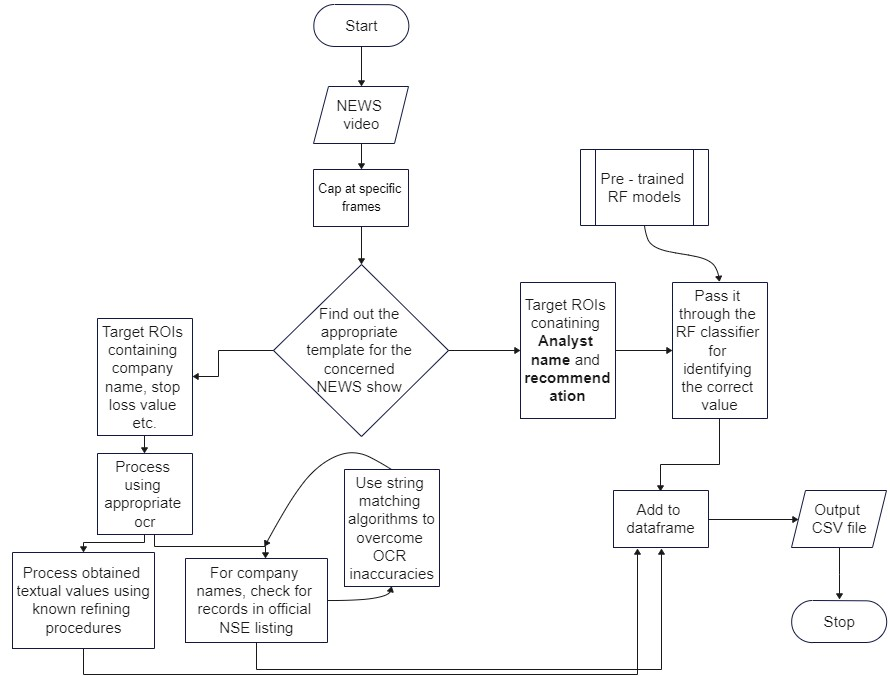
\includegraphics[scale=0.7]{chapter3/overall flow.jpeg}
  \caption{A flowchart representation of the entire methodology of the Python script}
  \label{fig:process_flow_python}
\end{figure}

\subsection{YoLov4} \label{yv4}

After the complete training of the dataset as described in the section \ref{train_test} is concluded, the execution of the {\fontfamily{qcr}\selectfont darknet.exe} command or the calling of a high-level library on a particular frame produces bounding boxes with appropriate coordinates, the class detected and the confidence score associated with each detection. There could be multiple detections in a frame, all of which would be returned. We may choose to somehow aggregate the confidence scores at the end to show an overall value of the percentage accuracy but it is completely optional. The important part of this process is \textbf{bounding box coordinates} which are obtained at the end. These would be sent into the OCR engine described in the next section.

\subsection{OCR models}

The deep learning models which follow the above YoLov4 models are the cascaded models working under the hood of the OCR engine. EasyOCR is the OCR chosen for this project, the reasons for which are described in section \ref{comp_ocr}. The two models are essentially a \textbf{text detection} model and a \textbf{language} model. It should be noted that there is only a single text detection model, however, there could be as many language detection models as you wish to detect. The common directory under which both these models would be stored is mentioned in the program as a path variable.

\begin{figure}[h]
  \centering
  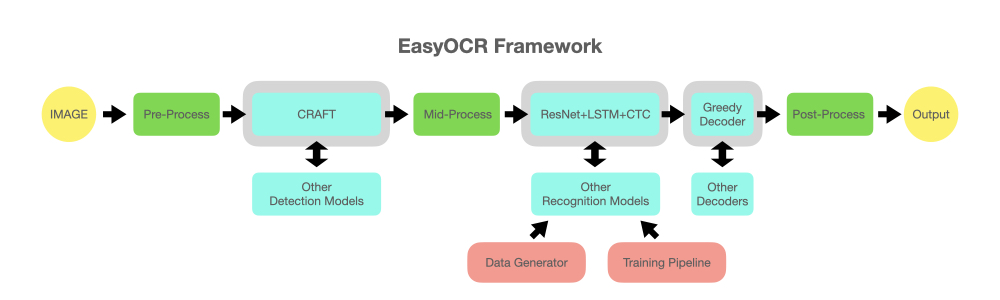
\includegraphics[scale=0.45]{chapter3/easyocr_framework.jpeg}
  \caption{The internal flow of EasyOCR}
  \label{fig:internal_ocr}
\end{figure}}

The methodology which is followed here is that the bounding box coordinates obtained from the previous step are converted to the form {\fontfamily{qcr}\selectfont [row\_start:row\_stop, column\_start:column\_stop]} which is applicable for any Python NumPy object or equivalently any image. EasyOCR then applies its capabilities only in the specific region as described by the set of converted coordinates. \par

The text detected would be having a variety of numerical values of stop-loss, target price, etc. All of them would essentially be linked to a single company (its listing symbol to be specific). This listing symbol forms the basis of creating keys in a Python dictionary which would all be unique. Any update to this dictionary would either add a key or update the values corresponding to a single key (or a listing symbol). It should be noted that the latter case is rare since analysts rarely give \textit{different} recommendations regarding the same company multiple times in a single broadcast. Then the concerned dictionary is converted to a Pandas data frame which is then finally converted to a CSV or an excel file as desired after appending a column containing a single date at the end. \par

This concludes the typical program flow for such a script. The following section describes, in brief, a difficult edge case wherein multiple recommendations may be detected in a single frame.

\subsubsection{Multiple recommendations in a frame}

Although we have not gone into the details of how the dataset on which the training is carried out in section \ref{train_test} looks like. It is known that there exist rare situations wherein multiple recommendations corresponding to distinct company shares are given in the same frame. In such cases, it is difficult to associate recommendations and other numerical values accurately with a company or its listing symbol. I have proposed a method below which is simple to follow and leads to substantial accuracy in such cases. \par

We are well aware that the multiple bounding boxes that are being returned by the YoLov4 model all lie along the same vertical axis. The only discerning feature is the limits of the bounding boxes along the $X$ - axis. Let $X_i$ and $X_j$ be the $X$ - axis limits for a detection containing a company name or its symbol. Let $x_i$ and $x_j$ be the $X$ - axis limits for a detection containing any of the following values: recommendation, target price, stop loss etc. The latter can be associated with the former if and only if either or both of the $X$ - axis limits of the latter are contained within the former. Precisely, the latter can be associated with the former if $x_{i} \geqslant X_{i}$ and (or)  $x_{j} \leqslant X_{j}$. It is driven by the reason that the latter is usually placed below the former in any NEWS show but with identical text size and width. \par

This concludes the discussion of the entire methodology involved in the project.

\chapter{Deployment in production} \label{chapter4}

\chapter{Results and discussions} \label{chapter5}

The following subsections shall discuss in detail, a variety of important comparisons which affect the project work, a brief overview of the methodologies learned, deviations from the ideal case (if any) and a creator’s road map for implementation of a similar project and other moderate and small details. It also has a section for the work which is being currently done at SEBI to improve the existing system. The initial two sections deal with metrics of accuracy and execution time across two different bases for comparison while the section that follows discusses why the metrics are chosen and defined as they are. \par

\section{Comparison between OCR models} \label{comp_ocr}

Both Tesseract and EasyOCR are sophisticated OCR engines and are available as open-source in their default versions. However, there exists an outsized number of differences in how they have been developed. While Tesseract \cite{Google2015} happens to be a quite superior alternative right from the beginning which can use even PDF files as input apart from the standard images, it turns out that there doesn’t exist any suitable interface with common programming languages (such as Python) which leads to a lot of problems. The first and foremost problem is that Tesseract needs to be set up in a way similar to how a particular program is set up on a remote server i.e. the \textit{only link} between a program using Tesseract and the actual engine is the file path. Customisations can be done nonetheless, but are difficult to implement due to the lack of a high-level interface. This leads directly to another issue: the Ezmeral MLOPs platform is set up on a legacy Centos 7.5 virtual machine cluster and won’t allow arbitrary software to be installed in it due to the presence of an enterprise-grade security architecture.  So it may be the better OCR engine in general, however, this use case is unsuitable for it.\par

EasyOCR offers as many capabilities \cite{Jaided2020} as Tesseract (\textit{sans} the direct processing of PDF files) and has a \textbf{high-level} library directly available for use in Python. This means that no preliminary server like set-up needs to be done to access the OCR engine, rather everything is on board once the program and all its imported modules are loaded onto memory. Hence, EasyOCR was chosen as the OCR for this project. \par

It should be noted that EasyOCR is a ready-to-use OCR that is invariant to colour images while the Tesseract documentation does say things about providing a greyscale image as input. This feature alone avoided a lot of extra image processing operations within the codebase. After using EasyOCR, the following changes took place:

\begin{itemize}
 \item The size of the codebase was greatly reduced (from $1400$ lines to less than $1000$ lines).
 \item The execution time dropped significantly (from $73$ to $14$ minutes: a reduction of $\approx 80\%$ on similar environments).
 \item Major improvements were not visible in accuracy although EasyOCR still managed to perform better ($A_{e} = 0.94375$ and $A_{e} = 0.95$ respectively).
\end{itemize}

Amongst all decoded values at the end of a particular run, the following results were obtained and are summarised below.

\begin{figure}[h]
  \centering
  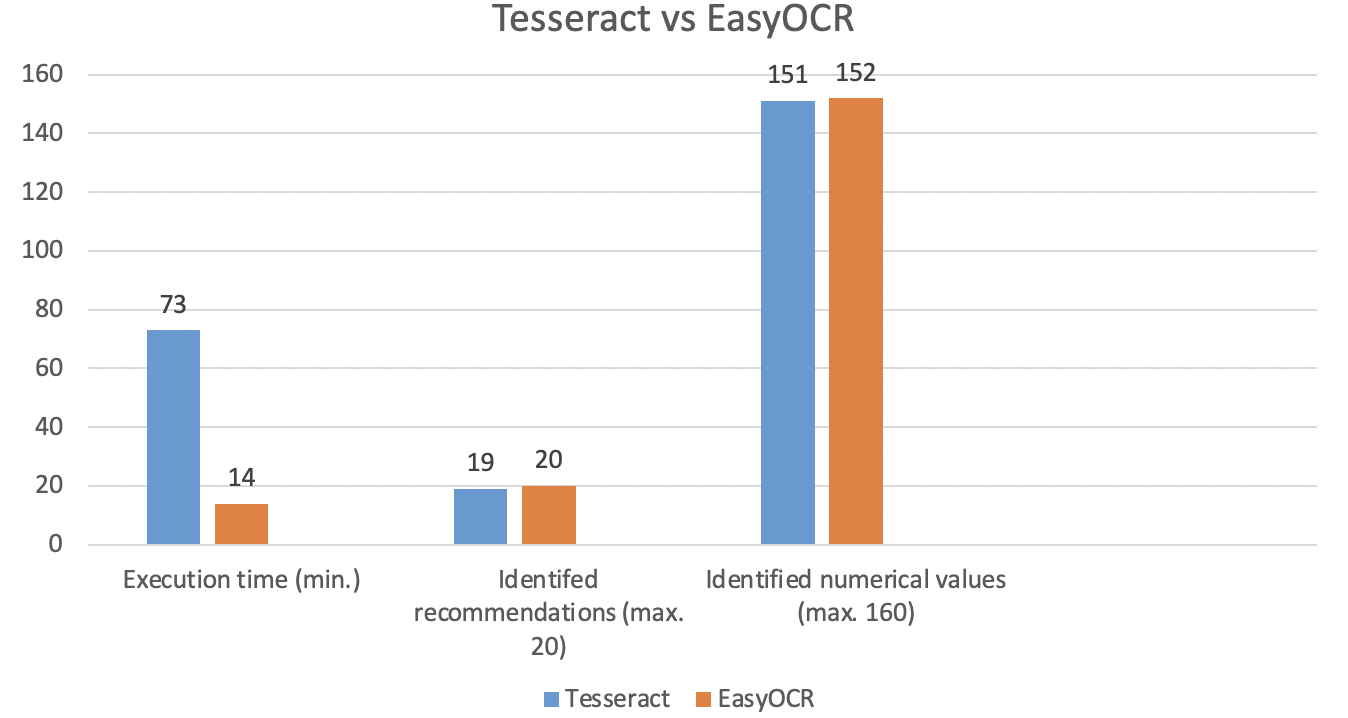
\includegraphics[scale=0.7]{chapter5/barchart.png}
  \caption{Comparison of Tesseract and EasyOCR for a sample $30$ minutes telecast}
  \label{fig:easy_vs_tess}
\end{figure}

Still, EasyOCR (and the project) benefits even further from a possible change in hardware configuration which is detailed in the following section.


\section{Comparison between hardware architectures}

It is a known fact that almost all deep learning systems (inclusive of computer vision models) benefit greatly from the presence of GPUs in the development environment. Although as of now the Ezmeral cluster doesn’t have GPU access, testing was still performed on a local workstation with an \href{ https://www.nvidia.com/en-in/geforce/20-series/}{RTX 2060} graphics card with the equivalent Nvidia \href{https://developer.nvidia.com/cuda-toolkit}{CUDA toolkit} installed. \par

It should be noted that \textbf{no execution environment} discussed earlier in chapter \ref{chapter4} had any mention of GPUs so there was a decrease in execution time by a large margin for the same test video. The decrease of roughly by a factor of $4.5$ w.r.t. to the closest competitor i.e. for execution recorded on a standalone VM. The reason for this was obvious: the documentation of EasyOCR mentions that their pipeline is more performant in the presence of a GPU \cite{Jaided}. The results are summarised in the form of a bar chart below.

\begin{figure}[h]
  \centering
  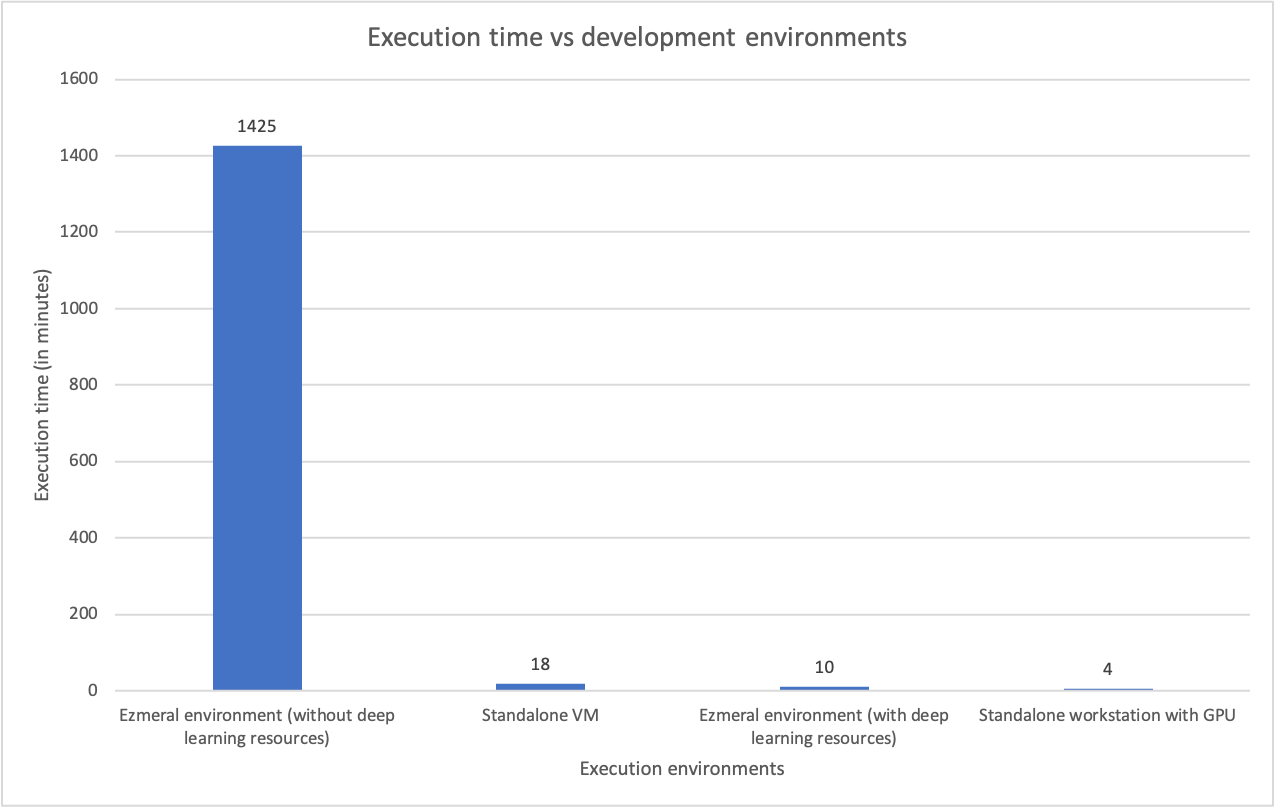
\includegraphics[scale=0.7]{chapter5/barchart2.png}
  \caption{A comparison of execution times across a variety of development environments with a variety of hardware configurations}
  \label{fig:hardware}
\end{figure}

\section{Current workflow progress and testing procedures}

\subsection{Workflow progress}

As stated in earlier chapters, the work at hand is to process a total of $7$ NEWS shows in their entirety (excluding only one for the lack of recommendations in it) to summarise all the recommendations being provided in them. This shall ensure that when more sophisticated anomaly detection models are run on them, the input (produced as an output from my project) is sufficient for them to run properly. Additionally, it should also be noted that the systems succeeding the ones used in this project also use several data cleaning procedures before arriving at a final output so a \textit{picture-perfect output is not necessary although desirable}. \par

The following table lists the shows on one side and the percentage of total videos of each show that has been processed.

\begin{table}[h]
 \def\arraystretch{1.5}
 \centering
 \caption{Batch workflow progress}
 \begin{tabular}{|c|c|}
  \hline
  NEWS show & Progress (in \%)\\
  \hline
  Buy Now Sell Now & $10$                   \\
  \hline
  Pehla Sauda & $25$                   \\
  \hline
  NSE Closing Bell & $10$                   \\
  \hline
  Bazaar Morning Call & $10$                   \\
  \hline
  Midcap Bazaar & $35$                 \\
  \hline
  Stock 20-20 & $100$                \\
  \hline
  Weekly Roundup & \textbf{Omitted}               \\
  \hline
 \end{tabular}
 \label{tab:news_prog}
\end{table}


\subsection{Testing procedures}

Usually, there are no clearly defined testing procedures for such custom projects in deep learning and computer vision. A typical testing procedure that was used to verify the authenticity and the accuracy of the output is that after filtering out frames at the FPS rate, the recommendations being made in a \textit{handful} of videos were noted down manually. This was then compared to the output obtained from the program. If there is a perfect match (which was mostly the case), then the output is deemed to be suitable otherwise \textbf{no separate improvements} are made midway in a batch processing workflow. The reason for this is two-fold:

\begin{enumerate}

 \item Batch processing workflows involve a very large number of videos at once, stopping them in between drastically decreases the efficiency of such workflows and the more important reason being

 \item Anomaly detection systems or models which follow this project already employ sufficient data cleaning procedures to obtain a reliable and usable output within tolerable error limits.

\end{enumerate}

\section{Accuracy}


\section{Inferences and learnings}

\subsection{Possible usage of only an OCR engine}

It would be worthwhile to reason why an OCR engine is not directly used on the extracted frames since it would detect the required text followed by which the programmer is supposed to consolidate it to a usable form. \par

The reason lies in the abilities of EasyOCR as an OCR engine which is both an advantage as well as a disadvantage. It should be known that, unlike Tesseract which uses page segmentation modes \cite{Rosebroc2021} to detect text in an image structurally arranged in specific configurations, EasyOCR doesn’t have any such facility. It directly returns a list of bounding box coordinates, the text detected along with a confidence score across the entire image \cite{Jaided}. The above is an illustration of what might happen if numerous texts were provided to EasyOCR on a signboard.

\begin{figure}[h]
  \centering
  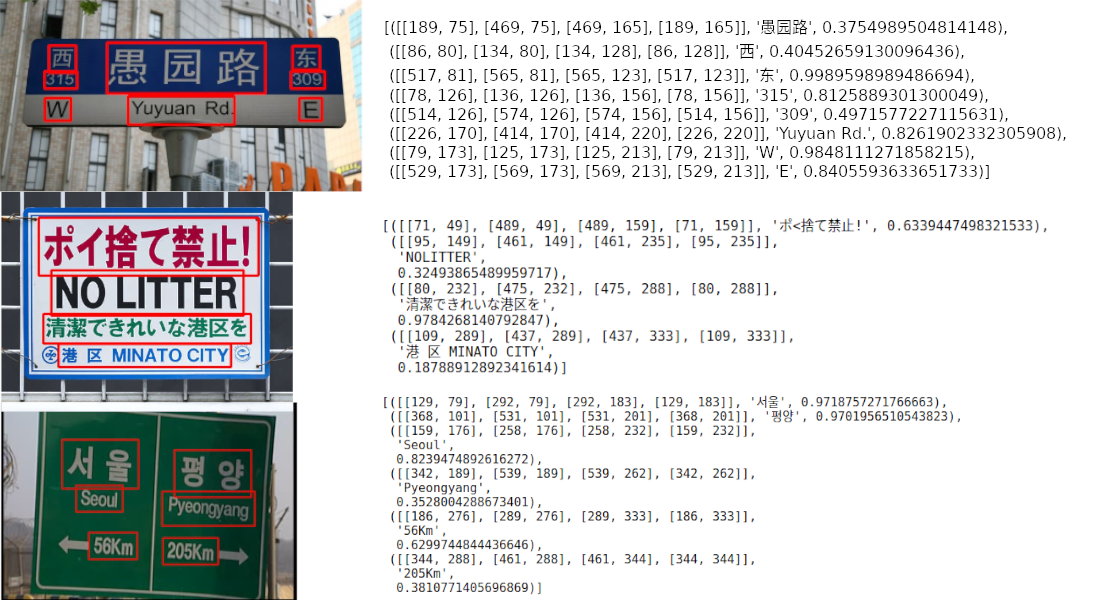
\includegraphics[scale=0.45]{chapter5/example2.png}
  \caption{Execution of EasyOCR on three signboards}
  \label{fig:easy_signboard}
\end{figure}

We would realise that all texts scattered throughout the image are returned, however, we are unable to draw any correlation between them at first look. This could prove to be a major challenge in this project wherein multiple related numerical and alphanumeric values are placed close to each other. In an extreme case where multiple recommendations are detected in the same frame, it would be very difficult to detect the mapping of the numerical values (such as stop-loss or target price) and the listing symbol of a company share. Hence, the choice of using an object detection model followed by an OCR engine.

\subsection{Procurement of data from a contractor}

It has been clearly stated in section \ref{vid_data} that the entirety of the video data was obtained from \href{clipbyte.com}{Clipbyte}. It would be worthwhile to argue that all videos could be directly downloaded from a platform like \href{youtube.com}{YouTube}. However, there are two major reasons for not doing so:
\begin{enumerate}
 \item All broadcasts of the concerned NEWS shows are not available on such video platforms and nor do the respective channels upload videos in a timed and orderly manner.

 \item There is no official way to download videos from such a platform so availing videos from such a platform by a Government regulatory body would imply improper means of accessing publicly available information in the situation wherein the InVestigations Department (IVD) of SEBI has to file a case against a suspected entity. The data source needs to be mentioned in the case file and hence a separate contractor has been tended for this job.

\end{enumerate}



\section{Accuracy, empirical accuracy and execution time}

A lot has been discussed about the various performance metrics used to evaluate object detection models in section \ref{metrics}, however, we still stick to the concept of simple empirical accuracy in the above two sections. The reason for the same is that there are multiple ML/DL models which are involved in this project. Each model has been designed (or is being used) to complete only a specific task amongst a large number of tasks that are to be executed sequentially. Each task involves different kinds of data and hence produces different kinds of output. \par

A simple e.g. being that the YoLo models discussed throughout the report output a set of mixed values as given in section \ref{brief_discuss} after taking in an image as an input. However, the OCR models that follow require an image as an input, but produce a textual output (i.e. of string datatype). These models within them have two deep learning models i.e. a \textit{text detection} and a \textit{language} model in a cascaded fashion out of which only the former receives an input in the form of an image while the second model deals with textual input and output. \par

Each of these models named above has its own set of accuracy metrics which may be discussed however, they would be irrelevant to the final output of the project. Hence, we have stuck to the concept of simple empirical accuracy which is defined by the set of values obtained at the end from the OCR and summarised in the CSV file and is defined as follows

\begin{equation}
\centering
A_{e} = 1 - \frac{No. \ of  \ NA \ values \ in \ the \ CSV}{Total \ no. \ of \ values \ in \ the \ CSV }
\end{equation}

\textit{Measuring execution time remains the same i.e. in seconds although at a couple of places wherein the execution time is large, seconds have been replaced by larger units of time}. \newpage

\section{Sample outputs}

This section has a couple of outputs for multiple NEWS shows for the sake of reference to the reader.

\begin{figure}[h]
  \centering
  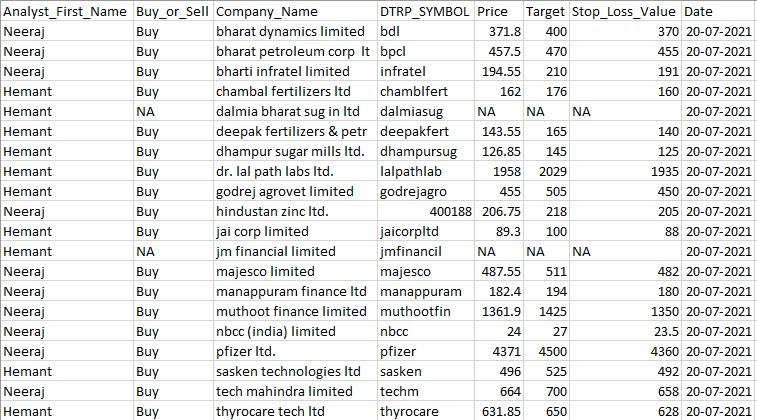
\includegraphics[scale=0.7]{chapter5/output csv.jpeg}
  \caption{The output file obtained for the broadcast of the NEWS show Stock 20-20 on 20/07/2021}
  \label{fig:out1}
\end{figure}

\begin{figure}[h]
  \centering
  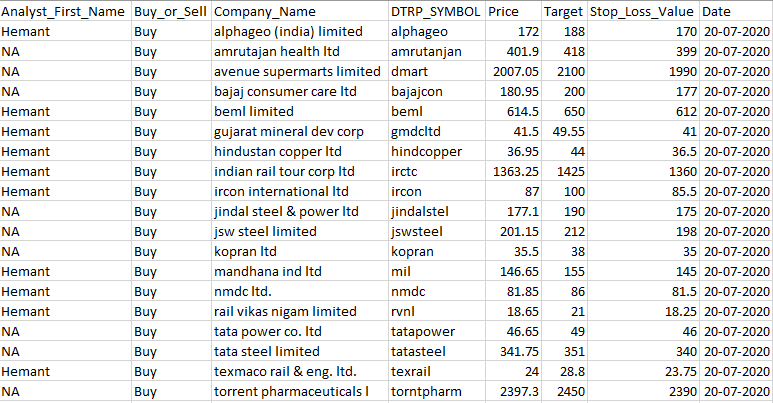
\includegraphics[scale=0.7]{chapter5/output2 csv.png}
  \caption{The output file obtained for the broadcast of the NEWS show Stock 20-20 on 20/07/2020}
  \label{fig:out2}
\end{figure} \newpage

\begin{figure}[h]
  \centering
  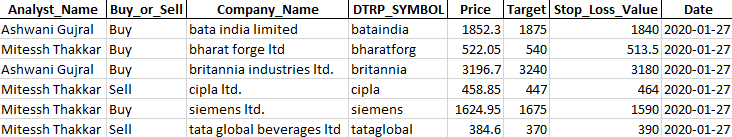
\includegraphics[scale=0.7]{chapter5/output3 csv.png}
  \caption{The output file obtained for the broadcast of the NEWS show CNBC TV18 on 27/01/2020}
  \label{fig:out3}
\end{figure}


\section{Future work}

The current system can be improvised in two different areas as given below. A workflow improvement can also be made.

\subsection{Accuracy and efficiency}

The current system does filtering at only the FPS rate which manages to reduce the number of frames under consideration to a much smaller value (a $25$\textsuperscript{th} of it to be precise). However, as we have seen in chapter \ref{chapter3}, the frame selection is still not inherently intelligent and still leads to the production of  $ \approx 1400$ frames on an average, amongst which frames would be manually selected for annotation. \par

Theoretically, we can say that for the problem statement at hand; there exists a program $P$ that extracts and processes exactly $N$ frames such that the total no. of recommendations being made, $R$ is contained in exactly $N$ keyframes. \par

To do so we can use an adaptive frame extraction algorithm \cite{adapt} which shall extract only the frames which are important to us. This method is based on matching histograms of successive frames, a correlation that exists amongst their colour channels, etc. This shall greatly reduce the number of frames to be processed at a time (apart from the already existing FPS rate filtering). This method, however, could be tending to fail because similar-looking frames \textit{need not be redundant} to us just because they appear close to each other in the actual video. In that case, we can go for an alternative approach wherein the frame numbers are output according to a simple implementation of any multi-output regressor \cite{Brownlee2020}. Since there could be inherent inaccuracies in the training of the same, we can use a spreading factor $\Delta$ which shall extract keyframes starting from ${f}_{k} - \Delta$ to ${f}_{k} + \Delta$ instead of just the frame $f_k$.

\subsection{Usability}

Currently, a two-part deployment and its necessity are deemed to be confusing to many SEBI officers who work in the surveillance department and don’t have any prior programming knowledge. Both these deployments could be integrated into a single native cross-platform desktop app developed either using \href{https://riverbankcomputing.com/software/pyqt/intro}{PyQt} or \href{electronjs.org}{Electron} which shall have an intuitive front end design and the same set of calling scripts as its backend. This shall help concerned officers keep track of ongoing workflows as well as use them when required without interfering with ongoing batch workflows and being aware of the complexity of the ML/DL code behind it.

\subsection{VM workflow} \label{future}

The landing server of SEBI Datalake would soon be modified in a way that it will subscribe to an MRSS feed on the Clipbyte platform wherein any new video once pushed shall automatically trigger a workflow. The VM workflow would be modified accordingly so that it either runs as a \href{https://en.wikipedia.org/wiki/Cron}{\textbf{cron}} job at scheduled intervals or it executes only when a new video is available for processing.

\chapter{Conclusions} \label{chapter6}

The various recommendations being made in NEWS shows were successfully detected (within tolerable error limits across a large size of input data), extracted and analysed for anomalies in the concerned process.  The input to the program script was simply the video file itself and the telecast date (which was reflected as it is in the last column). The end-user might download the summarised data as an excel or CSV file for further study. The final summarised data contained important fields like the \textbf{Name of the analyst}, the \textbf{share/stock} regarding which recommendation was being made: its \textbf{name} as well as its \textbf{listing symbol} in the appropriate exchange, the \textbf{actual recommendation} being made (buy, sell or hold), the \textbf{target price} and the associated \textbf{stop loss}.  A total of eight NEWS shows were processed in this manner wherein only a single NEWS show was skipped due to the lack of recommendations being made in the video dataset available to us. \par

As stated earlier in chapter \ref{chapter4}, the deployment of the above ML/DL models was parallelly done onto two separate systems, namely the HPE Ezmeral MLOPs server for single usage low-frequency requests and on a separate Linux virtual machine for large free-running batch processing workflows which would keep on running a single script continuously on a large dataset. \par

I got to learn a lot of things regarding machine learning, deep learning for computer vision, functioning of OCR engines, MLOPs deployment in different environments and as well as different guidelines which are to be followed for gathering a video dataset (e.g. sampling at FPS rate, annotating a dataset, partitioning the dataset properly etc.) and processing it accordingly for further analysis. Overall it turned out to be an entire knowledge enriching experience spanning a multitude of domains.




\newpage
\printbibliography
\addcontentsline{toc}{chapter}{Bibliography}


\end{document}
